\documentclass[border=10pt]{standalone}
\usepackage{tikz,amsmath}
\usetikzlibrary{arrows.meta}

% ========== 配色 ==========
\definecolor{hidFill}{RGB}{199,203,243}
\definecolor{hidLine}{RGB}{52,58,143}
\definecolor{inFill}{RGB}{183,224,177}
\definecolor{inLine}{RGB}{32,102,32}
\definecolor{orFill}{RGB}{250,224,180}
\definecolor{orLine}{RGB}{190,110,20}
\definecolor{yeFill}{RGB}{252,240,180}
\definecolor{yeLine}{RGB}{180,150,20}
\definecolor{outFill}{RGB}{243,199,199}
\definecolor{outLine}{RGB}{143,52,52}
\definecolor{gyFill}{RGB}{225,225,225}
\definecolor{gyLine}{RGB}{100,100,100}

\begin{document}
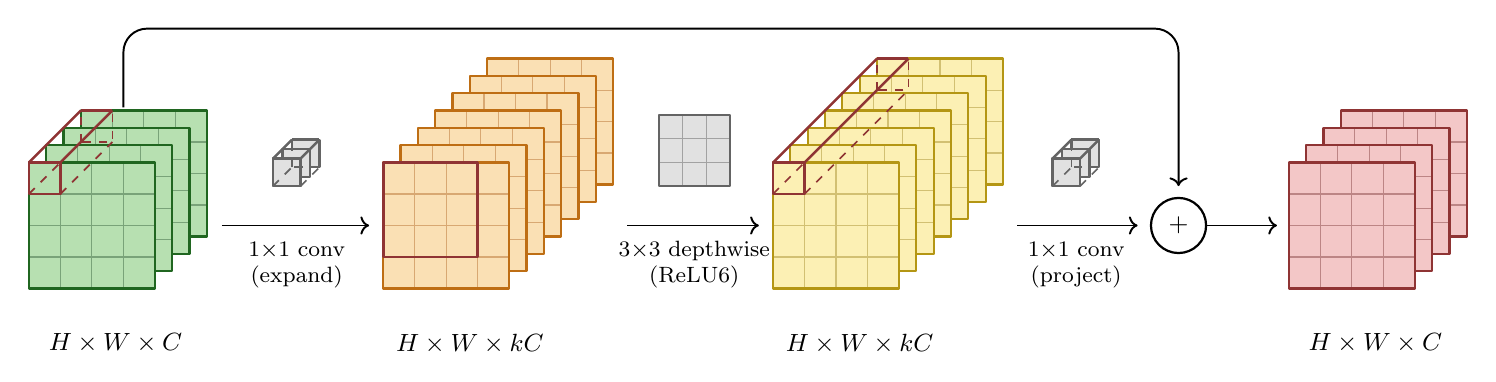
\begin{tikzpicture}[
    font=\small, line join=round,
    every node/.style={inner sep=0pt, outer sep=0pt, align=center},
    arr/.style={->, line width=.7pt}
  ]

  % ========== 宏 ==========
  \newcommand{\gridbox}[5]{%
    \fill[#5Fill] (#1,#2) rectangle (#1+#3*#4, #2+#3*#4);
    \draw[step=#4, #5Line!60, line width=.4pt, shift={(#1,#2)}] (0,0) grid (#3*#4, #3*#4);
    \draw[#5Line, thick] (#1,#2) rectangle (#1+#3*#4, #2+#3*#4);
  }
  \newcommand{\fstack}[4]{%
    \foreach \k in {#4,...,1}{%
      \gridbox{#1+.22*\k}{#2+.22*\k}{4}{.4}{#3}%
    }%
    \gridbox{#1}{#2}{4}{.4}{#3}%
  }
  \newcommand{\winbox}[3]{%
    \draw[outLine, dashed, line width=.6pt] (#1+#3,#2+#3) rectangle ++(.4,.4);
    \draw[outLine, line width=.9pt] (#1+#3,#2+.4+#3) -- (#1+.4+#3,#2+.4+#3);
    \draw[outLine, dashed, line width=.6pt] (#1,#2) -- (#1+#3,#2+#3) (#1+.4,#2) -- (#1+.4+#3,#2+#3);
    \draw[outLine, line width=.9pt] (#1,#2) rectangle ++(.4,.4);
    \draw[outLine, line width=.9pt] (#1,#2+.4) -- (#1+#3,#2+.4+#3) (#1+.4,#2+.4) -- (#1+.4+#3,#2+.4+#3);
  }
  \newcommand{\kbox}[2]{%
    \gridbox{#1+.24}{#2+.24}{1}{.35}{gy}
    \gridbox{#1+.12}{#2+.12}{1}{.35}{gy}
    \gridbox{#1}{#2}{1}{.35}{gy}
    \draw[gyLine, dashed, line width=.6pt] (#1+.24,#2+.24) rectangle ++(.35,.35);
    \draw[gyLine, line width=.9pt] (#1+.24,#2+.59) -- (#1+.59,#2+.59);
    \draw[gyLine, dashed, line width=.6pt] (#1,#2) -- (#1+.24,#2+.24) (#1+.35,#2) -- (#1+.59,#2+.24);
    \draw[gyLine, line width=.9pt] (#1,#2) rectangle ++(.35,.35);
    \draw[gyLine, line width=.9pt] (#1,#2+.35) -- (#1+.24,#2+.59) (#1+.35,#2+.35) -- (#1+.59,#2+.59);
  }

  % ========== 各阶段特征图（无 SE，四堆）==========
  \fstack{0}{0.7}{in}{3}
  \fstack{4.5}{0.7}{or}{6}
  \fstack{9.45}{0.7}{ye}{6}
  \fstack{16.0}{0.7}{out}{3}

  % ========== 箭头 1：1x1 expand + ReLU6 ==========
  \winbox{0}{1.9}{.66}
  \draw[arr] (2.45,1.5) -- (4.32,1.5);
  \kbox{3.1}{2.0}
  \node[font=\footnotesize] at (3.4,1.0) {1$\times$1 conv\\(expand)};

  % ========== 箭头 2：3x3 depthwise + ReLU6 ==========
  \draw[outLine, line width=1pt] (4.5,1.1) rectangle (5.7,2.3);
  \draw[arr] (7.6,1.5) -- (9.27,1.5);
  \gridbox{8.0}{2.0}{3}{.3}{gy}
  \node[font=\footnotesize] at (8.45,1.0) {3$\times$3 depthwise\\(ReLU6)};

  % ========== 箭头 3：1x1 linear project ==========
  \winbox{9.45}{1.9}{1.32}
  \draw[arr] (12.55,1.5) -- (14.08,1.5);
  \kbox{13.0}{2.0}
  \node[font=\footnotesize] at (13.3,1.0) {1$\times$1 conv\\(project)};

  % ========== 相加节点 + 输出 ==========
  \node[circle, draw=black, line width=.8pt, fill=white, minimum size=.7cm,
        font=\small] (plus) at (14.6,1.5) {$+$};
  \draw[arr] (14.95,1.5) -- (15.85,1.5);

  % ========== 残差连接（圆角，同尺寸同通道时）==========
  \draw[arr, line width=.7pt, rounded corners=3mm]
    (1.2,3.0) -- (1.2,4.0) -- (14.6,4.0) -- (14.6,2.0);

  % ========== 底部标签 ==========
  \node at (1.1,-0) {$H\times W\times C$};
  \node at (5.6,-0) {$H\times W\times kC$};
  \node at (10.55,-0) {$H\times W\times kC$};
  \node at (17.1,-0) {$H\times W\times C$};

\end{tikzpicture}
\end{document}